




\begin{frame}
    \frametitle{Stochastic Processes}
    \begin{itemize}
        \item A stochastic process is defined as a family of random variables ${X(t),t\in T}$.
        \item The parameter $t$ usually represents time, so $X(t)$ denotes the value assumed by the random variable at time $t$
        \item If the index set is discrete, e.g., $T = {0, 1, 2, . . .}$, then we have a discrete-time parameter stochastic 
        process; otherwise, if $T$ is continuous
        \item The values assumed by the random variables $X(t)$ are called states
    \end{itemize}
\end{frame}


\begin{frame}
    \frametitle{Stochastic Process}
    \begin{itemize}
        \item It is often possible to represent the behavior of a system, physical 
        or mathematical, by describing all the different states it may occupy (possibly 
        an infinite number) and by indicating how it moves among these states.
        \item These transitions are assumed to occur instantaneously
        \item If the future evolution of the system depends only only
        its current state and not on its past history, then the system may be represened
        by a \textbf{Markov Process}
    \end{itemize}
\end{frame}


\begin{frame}
    \frametitle{Stochastic Process}
    \begin{itemize}
        \item \textbf{nonstationary:} A process whose evolution depends on the time at which 
        it is initiated is said to be nonstationary.

        \item \textbf{stationary:} when it is invariant under an arbitrary shift of the time origin. 
        Mathematically, we say that a stochastic process is stationary if its joint distribution 
        is invariant to shifts in time, i.e., if for any constant $\alpha$,

        $$P[X(t_1)\leq x_1, X(t_2)\leq x_2, ..., X(t_n)\leq x_n] = $$
        $$P[X(t_1+\alpha)\leq x_1, X(t_2+\alpha)\leq x_2, ..., X(t_n+\alpha)\leq x_n]$$
    
        for all $n$ and all $t_i$ and $x_i$ with $i = 1, 2, . . . , n$.
    \end{itemize}
\end{frame}



\begin{frame}
    \frametitle{Markov Process}
    \begin{itemize}
        \item A Markov process is a stochastic process whose conditional probability 
        distribution function satisfies the Markov or \textbf{memoryless property}. 
        
        \item Consequently, we may define discrete-time Markov chains (DTMCs) and continuous-time 
        Markov chains (CTMCs) as well as discrete-time Markov processes and continuous-time Markov processes.
    \end{itemize}
\end{frame}


\section{Discrete-Time Markov Chains}


\begin{frame}
    \frametitle{Discrete-Time Markov Chains}

    \begin{definition}
        Formally, a discrete-time Markov chain ${X_n , n = 0, 1, 2,...}$ is a stochastic process that 
        satisfies the following relationship, called the Markov property.
        For all natural numbers $n$ and all states $x_n$,

        $$P[X_{n+1}=x_{n+1}|X_{n}=x_{n},X_{n-1}=x_{n-1},...,X_{0}=x_{0}] = $$
        $$P[X_{n+1}=x_{n+1}|X_{n}=x_{n}]$$
    \end{definition}


    \begin{itemize}
        \item The future is independend of the past given the present;
        \item {\color{red}To move to the next state we only need to know the current state}
    \end{itemize}

\end{frame}


\begin{frame}
    \frametitle{Transition Probability Matrix}
    \begin{itemize}
        \item To simplify the notation,rather than using $x_i$ to represent the states of a Markov chain, 
        henceforth we shall use single letters, such as $i$, $j$, and $k$.

        \item The conditional probabilities $P[X_{n+1} = x_{n+1}|X_n = x_n]$, now written 
        as $P[X_{n+1} = j|X_n = i]$, are called the single-step transition probabilities, or 
        just the transition probabilities, of the Markov chain.

        $$p_{ij}(n) = P[X_{n+1} = j|X_n = i]$$

        \item The matrix $P(n)$, formed by placing $p_{ij}(n)$ in row $i$ and column $j$, for all $i$ and $j$, is called the
        \textbf{transition probability matrix}.

    \end{itemize}
\end{frame}



\begin{frame}
    \frametitle{Transition Probability Matrix}
    \begin{itemize}
        \item A Markov chain is said to be \textbf{(time-)homogeneous} if for all states $i$ and $j$
        \small
        $$P[X_{n+1} = j|X_n = i] = P[X_{n+m+1} = j|X_{n+m} = i]$$

        for $n = 0,1,2,...$ and $m\leq 0$. To elaborate on this a little further, we have, for a 
        homogeneous Markov chain,
        \small
        $$p_{ij} = P[X_1=j|X_0=i] = P[X_2=j|X_1=i] = ...$$

        and we have replaced $p_{ij}(n)$ with $p_{ij}$ , since transitions no longer depend on $n$.

        \item For a \textbf{nonhomogeneous} Markov chain,

    \end{itemize}
\end{frame}


\begin{frame}
    \frametitle{Transition Probability Matrix: Example}
    \begin{figure}
        \centering
        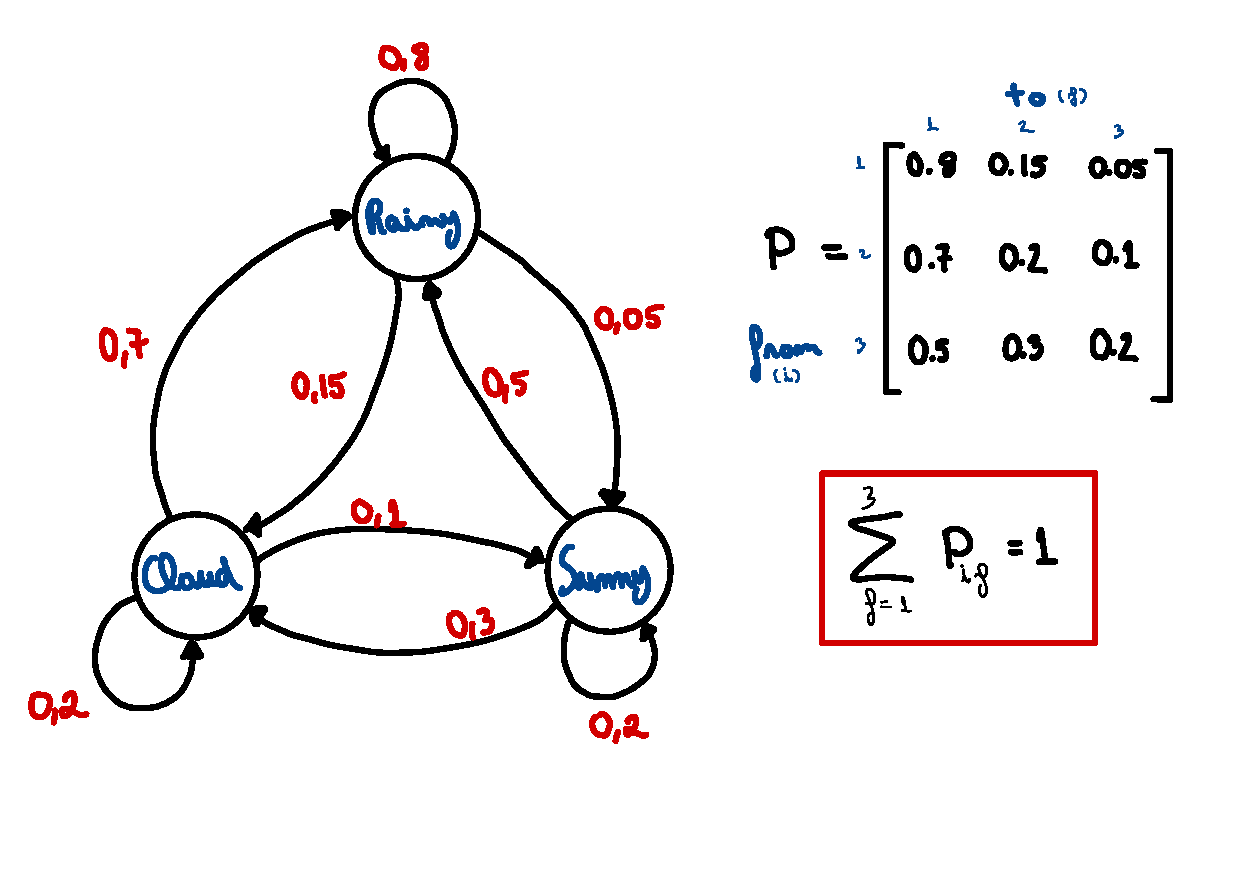
\includegraphics[width=0.95\textwidth]{slides/figures/markov_chain_example.pdf}
    \end{figure}
\end{frame}


\begin{frame}
    \frametitle{k-Dependent Markov Chains}
    \begin{itemize}

        \item Suppose, in the Belfast weather example, we are told that, if there are two rainy days in a row,
        What is the probabilities that the following day is rainy, cloudy, or sunny? 

        \item The probability of transitions from a rainy day depend not only on the fact that today 
        it is raining, but also on the weather yesterday (\textbf{Non-markov process})

        \item However, at the cost of increasing the number of states, it can be made into a Markov chain.

        \item If a stochastic process has s states and is such that transitions from each state depend on the history 
        of the process during the two prior steps, then a new process (k-dependent process) 
        consisting of $s^2$ states may be defined as a Markov chain.
    \end{itemize}
\end{frame}


\begin{frame}
    \frametitle{k-Dependent Markov Chains: Example}
    \begin{figure}
        \centering
        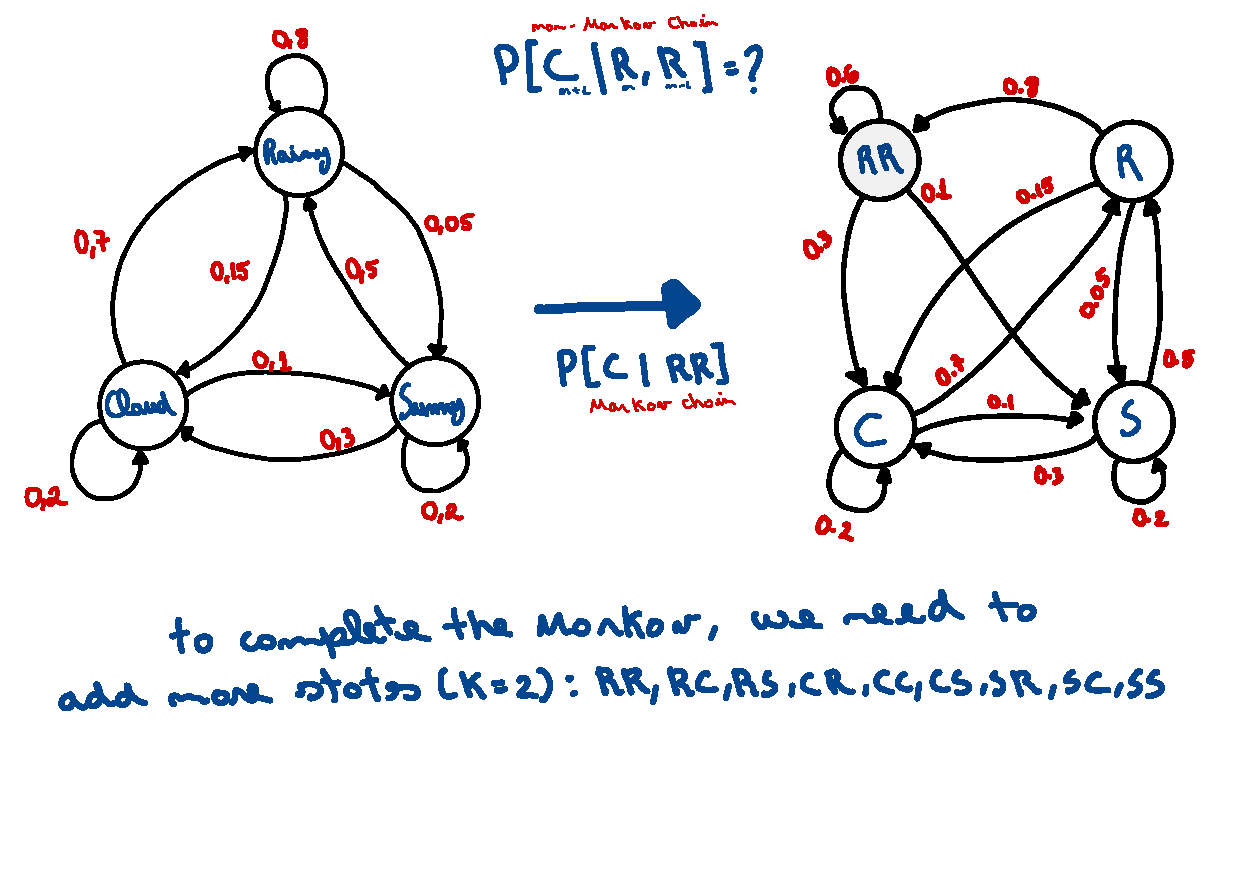
\includegraphics[width=0.95\textwidth]{slides/figures/markov_chain_k_dependent_example.pdf}
    \end{figure}
\end{frame}




\begin{frame}
    \frametitle{The Chapman-Kolmogorov Equations}
        We would now like to answer questions such as how to find the probability that it is cloudy two 
        days from now, given that it is sunny today.
        \begin{figure}
            \centering
            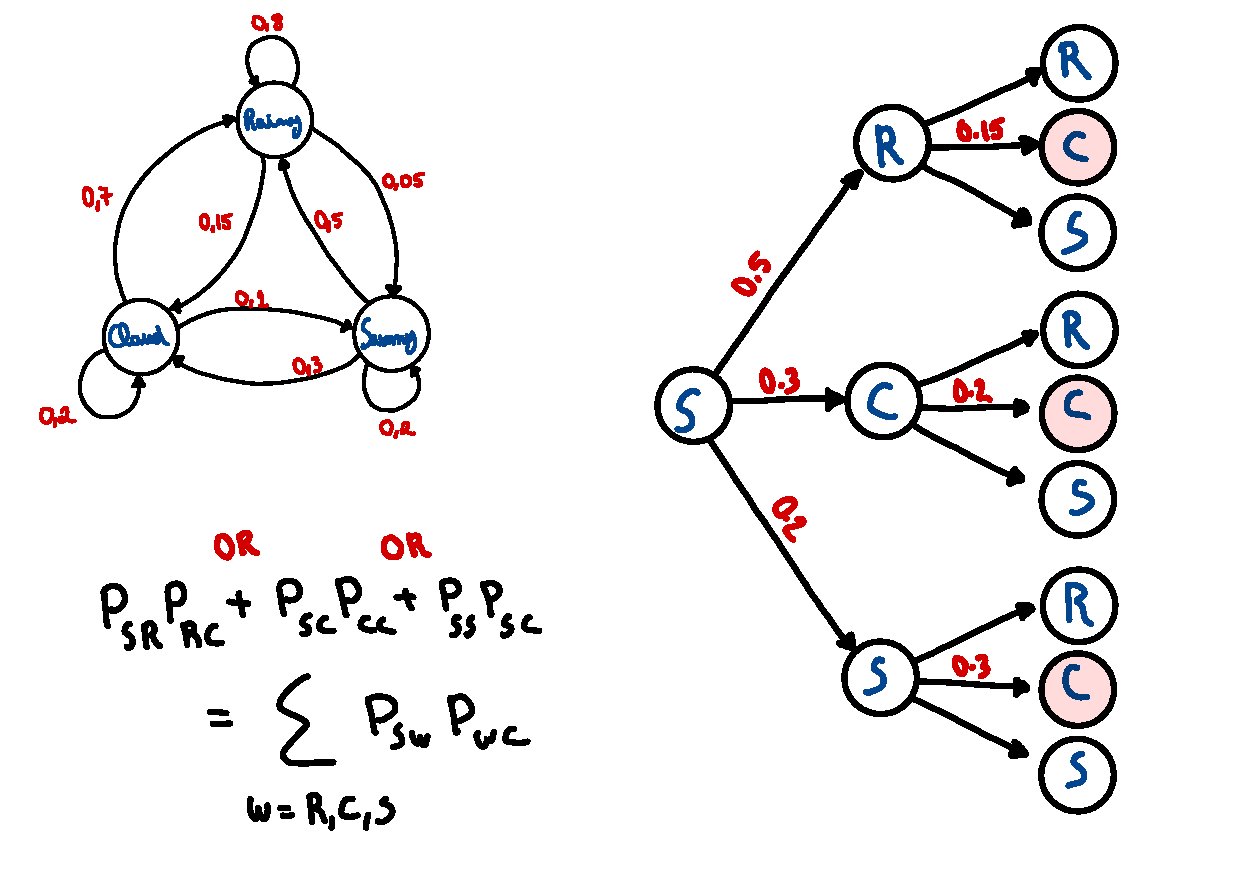
\includegraphics[width=0.8\textwidth]{slides/figures/markov_chain_2_steps_after_example.pdf}
        \end{figure}
\end{frame}


\begin{frame}
    \frametitle{The Chapman-Kolmogorov Equations}
        We would now like to answer questions such as how to find the probability that it is cloudy two 
        days from now, given that it is sunny today.
        \begin{figure}
            \centering
            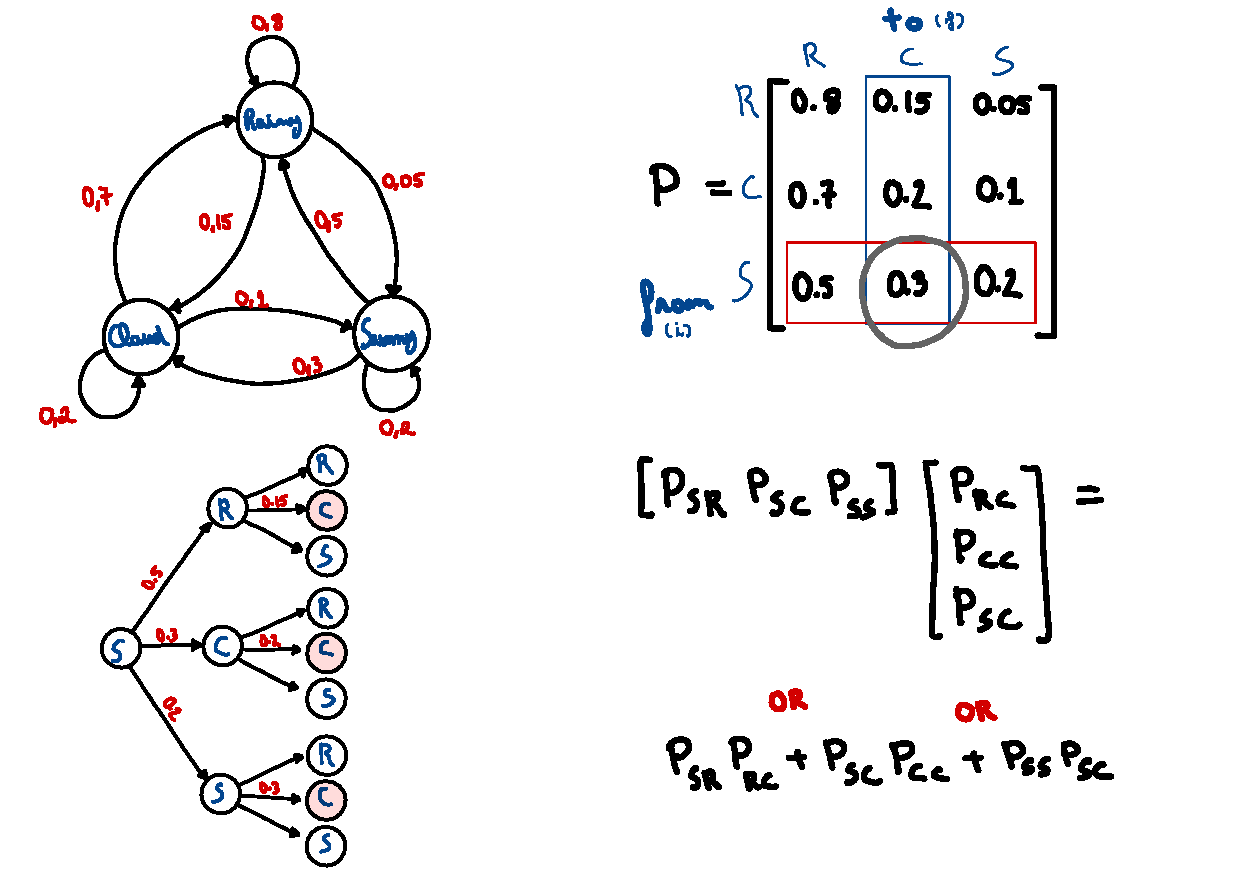
\includegraphics[width=0.8\textwidth]{slides/figures/markov_chain_2_steps_after_example_part_two.pdf}
        \end{figure}
\end{frame}


\begin{frame}
    \frametitle{The Chapman-Kolmogorov Equations}
    \begin{itemize}

        \item The probability that, two days from now, the weather is $w_2$ where w2 ∈ {R, C, S}, is obtained by
        forming the inner product of row $w_1$ with column $w_2$. All nine different possibilities constitute the
        elements of the matrix $P^2$.

        \item In a more general context, the $i,j$ element of the square of a transition probability matrix of 
        a homogeneous discrete-time Markov chain is the probability of being in state $j$ two time steps 
        from now, given that the current state is state $i$.

        \item In a similar fashion, the elements of $P^3$ give the conditional probabilities three steps from now, and so on. 
    \end{itemize}
\end{frame}



\begin{frame}
    \frametitle{The Chapman-Kolmogorov Equations: Proof}
        \begin{figure}
            \centering
            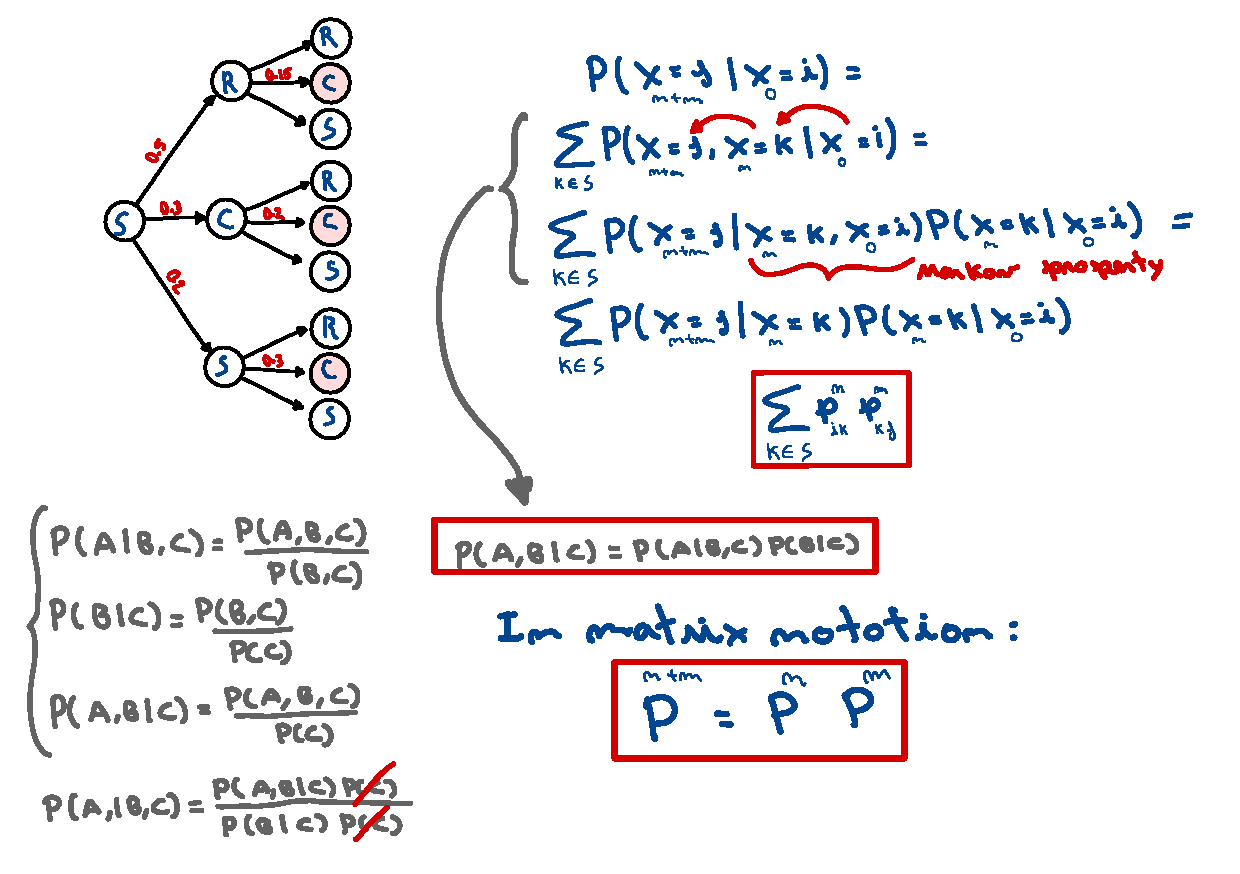
\includegraphics[width=0.95\textwidth]{slides/figures/chapman_kolmogorov_proof.pdf}
        \end{figure}
\end{frame}


\begin{frame}
    \frametitle{Classification of States: Definitions}
    \begin{itemize}

        \item Given two states of $i$ and $j$, a \textbf{path} from $i$ to $j$ is a sequence of 
        transitions that begins in $i$ and ends $j$, such that each transition in the sequence
        has a positive probability of occurring.

        \item A state $j$ is \textbf{reachable} from state $i$ if there is a path leading from $i$ to $j$.

        \item Two states $i$ and $j$ are said to \textbf{communicate} if $j$ is reachable
        from $i$, and $j$ is reachable from $j$.

        \item A set of states $S$ in a Markov chain is a \textbf{closed set} if no state outside
        of $S$ is reachable from any state in $S$.

    \end{itemize}
\end{frame}

\begin{frame}
    \frametitle{Classification of States: Example (1)}
        \begin{figure}
            \centering
            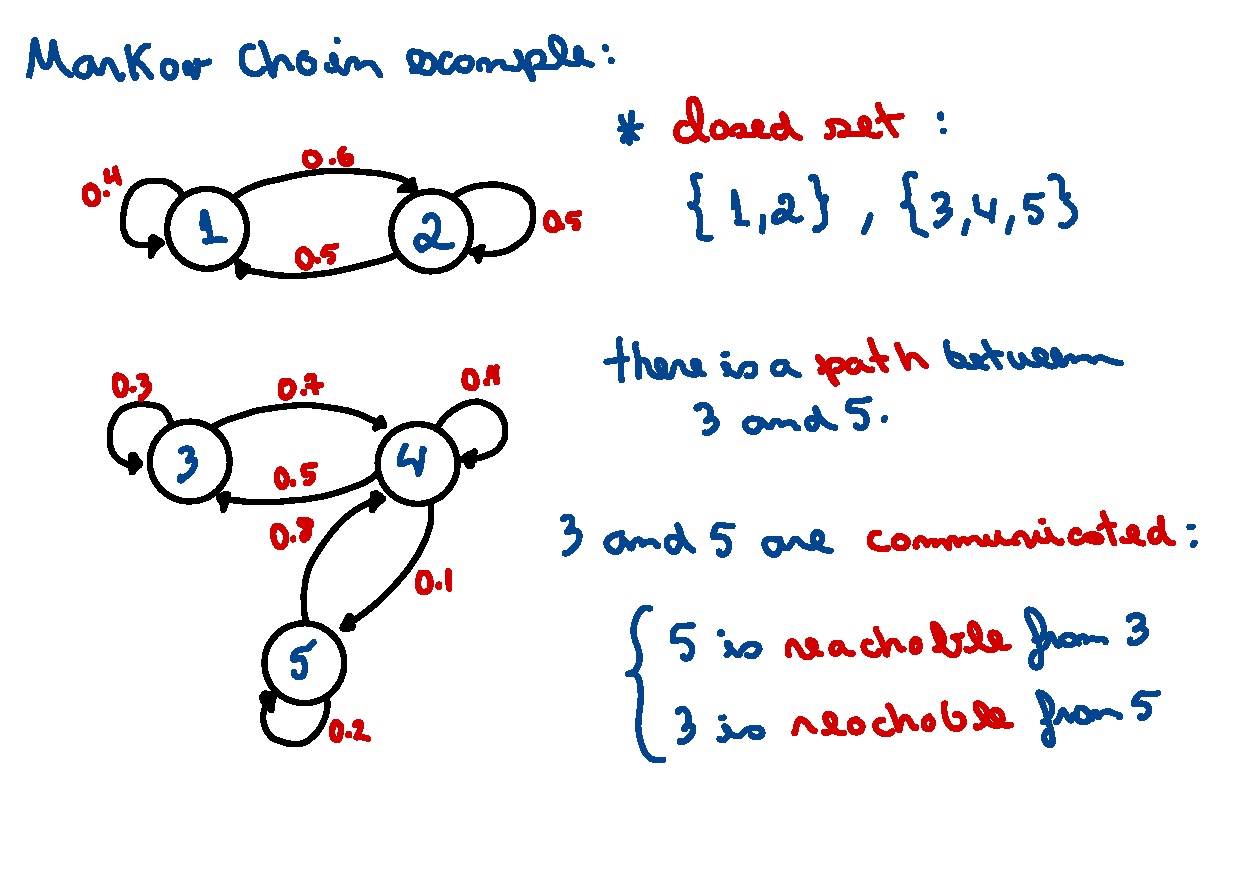
\includegraphics[width=0.95\textwidth]{slides/figures/classification_states_example_one.pdf}
        \end{figure}
\end{frame}

\begin{frame}
    \frametitle{Classification of States: Definitions}
    \begin{itemize}

        \item A state $i$ is an \textbf{absorbing state} if $p_{ii} = 1$.

        \item A state $i$ is a \textbf{transient state} if there exists a state $j$
        that is reachable from $i$, but the state $i$ is not reachable from $j$.


        \item If a state is not transient, it is called a \textbf{recurrent state}.

        \item A state $i$ is \textbf{periodic} with period $k>1$ if $k$ is 
        the smallest number such that all paths leading from state $i$ back 
        to state $i$ have a length that is a multiple of $k$. If a recurrent state
        is not periodic, it is referred to as \textbf{aperiodic}.
    \end{itemize}
\end{frame}

\begin{frame}
    \frametitle{Classification of States: Example (2)}
        \begin{figure}
            \centering
            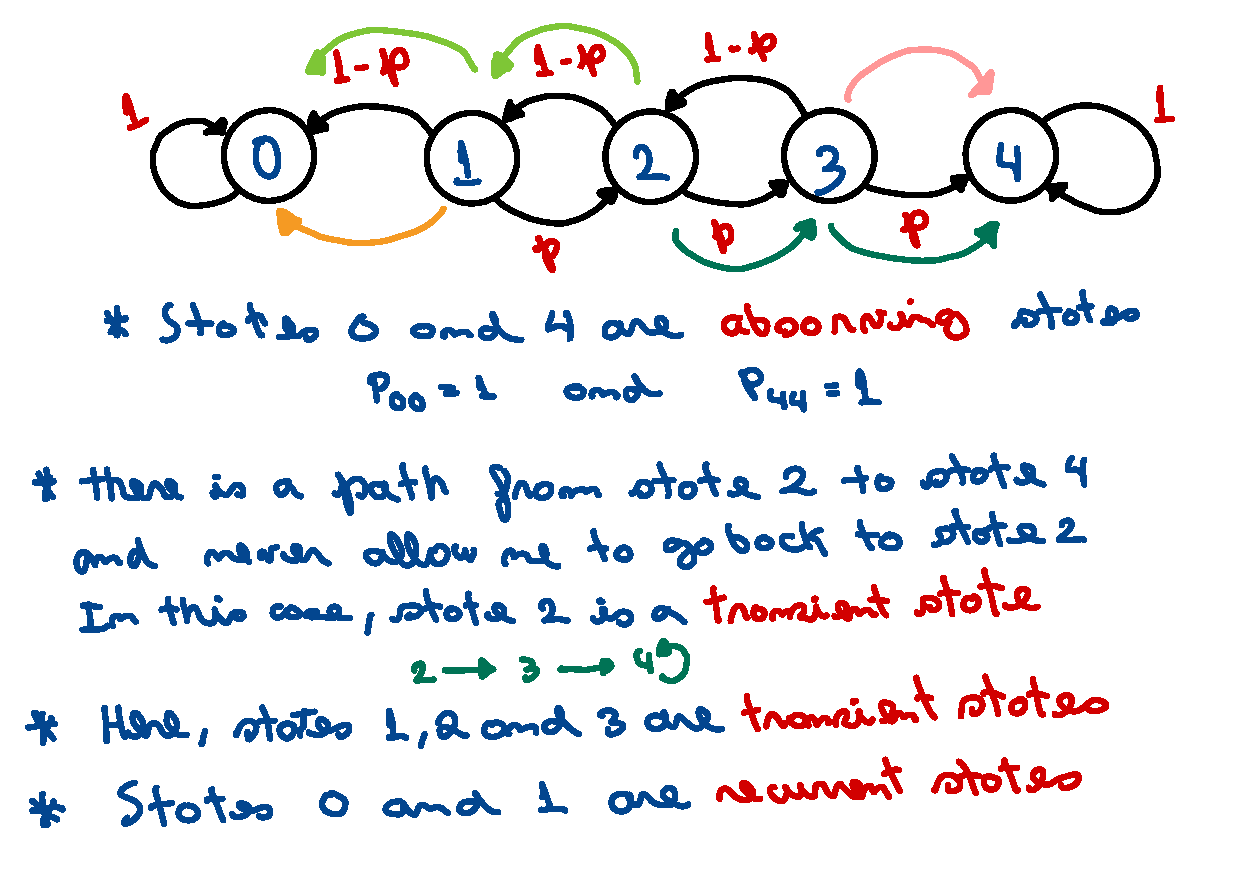
\includegraphics[width=0.95\textwidth]{slides/figures/classification_states_example_two.pdf}
        \end{figure}
\end{frame}

\begin{frame}
    \frametitle{Classification of States: Example (3)}
        \begin{figure}
            \centering
            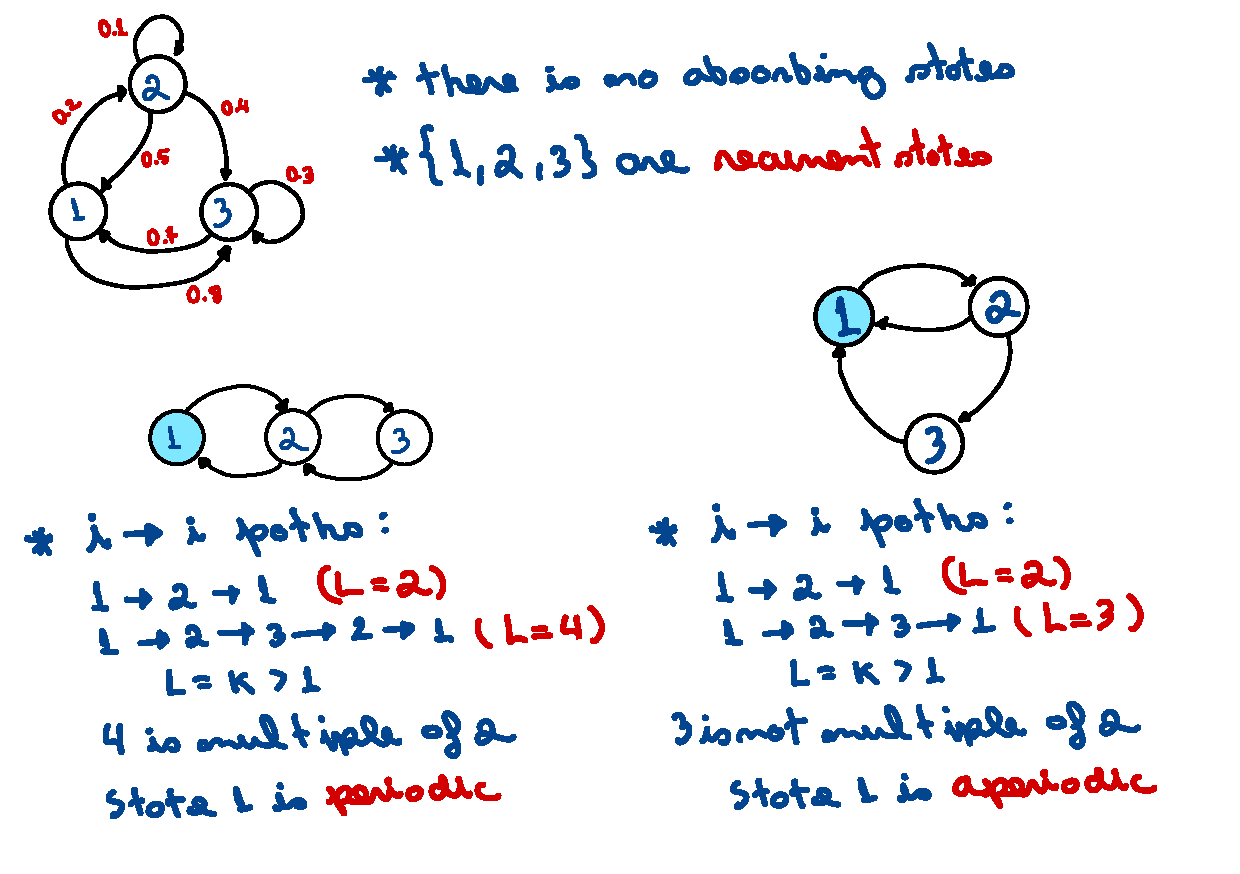
\includegraphics[width=0.95\textwidth]{slides/figures/classification_states_example_three.pdf}
        \end{figure}
\end{frame}


\begin{frame}
    \frametitle{Probability Distributions}
        \begin{itemize}
            \item Let's shall denote $\pi_i(n)$ the probability that a Markov chains is in state $i$ at step $n$.
            $$\pi_i(n) = P(X_n = i)$$

            \item The state probabilities at any time step n may be obtained from a knowledge of the initial 
            probability distribution (at time step 0) and the matrix of transition probabilities. We have, from 
            the theorem of total probability,
            \small

            $$\pi_i(n) = \sum_{k\in S} P(X_n = i| X_0 = k)P(X_0 = k) $$

            \item The probability that the Markov chain is in state i at step n is therefore given by

            $$\pi_i(n) = \sum_{k\in S} p_{ki}^n\pi_k(0)$$
        \end{itemize}
\end{frame}

\begin{frame}
    \frametitle{Probability Distributions}
        \begin{figure}
            \centering
            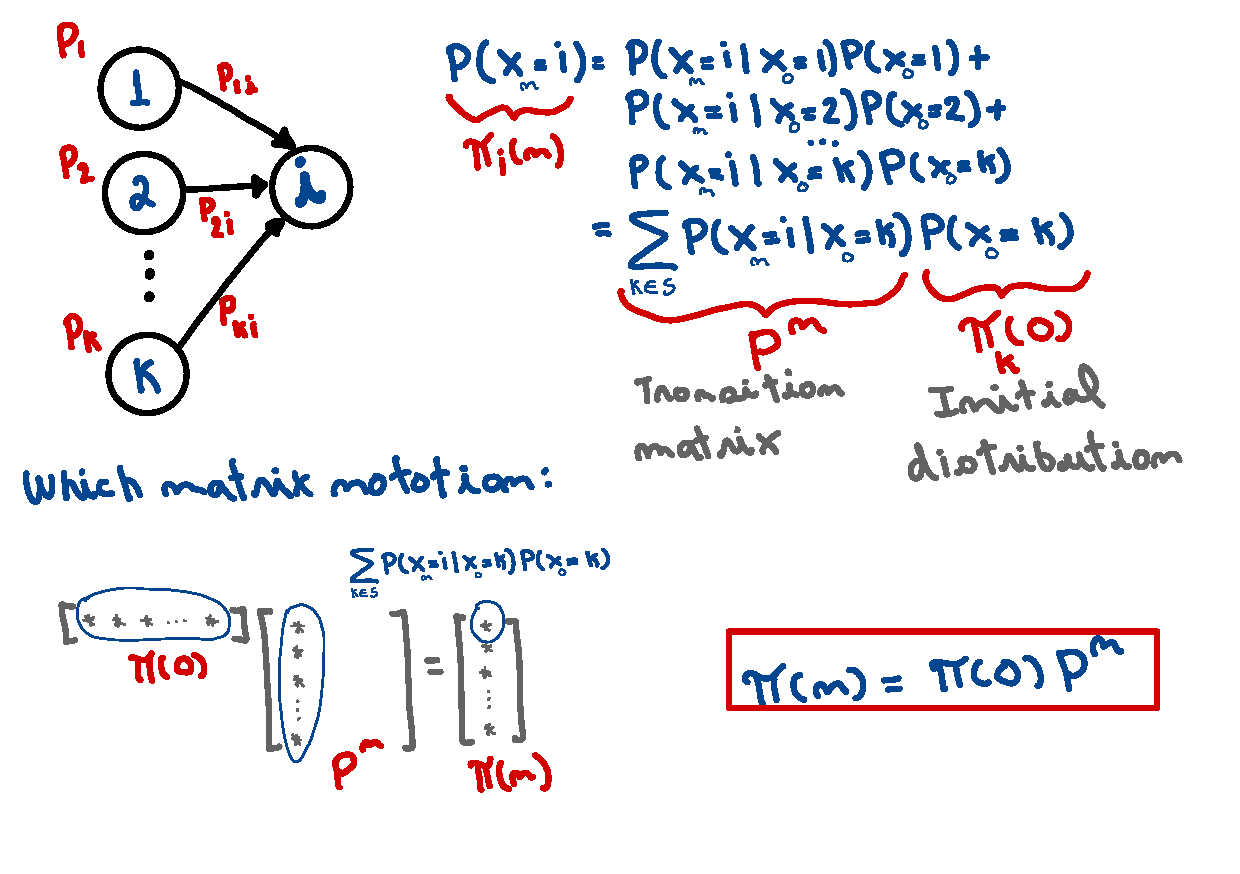
\includegraphics[width=0.95\textwidth]{slides/figures/pi_dist_proof.pdf}
        \end{figure}
\end{frame}


\begin{frame}
    \frametitle{Probability Distributions: Stationary distribution}
        \begin{definition}
            Let $P$ be the transition probability matrix of a discrete-time Markov chain, and let 
            the vector $z$, whose elements $z_j$ denote the probability of being in state $j$, be a probability 
            distribution. Then $z$ is said to be a stationary distribution if and only if $zP = z$.
        \end{definition}

        In other words, if $z$ is chosen as the initial probability distribution, i.e., $\pi_j(0) = z_j$
        for all then for all $n$, we have {\color{red}$\pi_j(n) = z_j$}.
\end{frame}




\begin{frame}
    %\frametitle{Probability Distributions: Stationary distribution when $n\rightarrow\infty$}
        \begin{definition}[Limiting distribution]
            Let $P$ be the transition probability matrix of a homogeneous discrete-time 
            Markov chain and let $\pi(0)$ be an initial probability distribution. If the limit
            $$\lim_{n \to\infty} P^n$$
            exists, then the probability distribution
            $$\pi = \lim_{n \to\infty}\pi(n) = \lim_{n \to\infty}\pi(0)P^n = \pi(0)\lim_{n \to\infty}P^n$$
        \end{definition}

        \begin{definition}[Steady-state distribution]
            A limiting distribution $\PI$ is a steady-state distribution if it converges, independently of 
            the initial starting distribution $\pi(0)$, to a vector whose components are strictly 
            positive (i.e., $\pi_i>0$ for all states $i$) and sum to 1. If a steady-state distribution 
            exists, it is unique.
        \end{definition}

\end{frame}



\begin{frame}
    \frametitle{Probability Distributions: Steady-state}
        \begin{itemize}
            \item Component i of a steady-state distribution is the probability that a random observer sees the Markov 
            chain in state i after the process has evolved over a long period of time.


            \item Steady-state distributions are also called equilibrium distributions and long-run distributions, to 
            highlight the sense that the effect of the initial state distribution $\pi(0)$ has disappeared.


            \item Steady-state distribution is the unique vector $pi$ that satisfies (Limiting distribution)
            \small
            $$\pi = \pi(0)\lim_{n \to\infty}\pi(0)P^n = \pi(0)\lim_{n \to\infty}\pi(0)P^(n+1) = $$
            $$\left[\pi(0)\lim_{n \to\infty}\pi(0)P^n\right]P = \pi~P$$

        \end{itemize}
\end{frame}


\begin{frame}
    \frametitle{Probability Distributions: Steady-state}
        \begin{itemize}
            \item The equations $\pi = \pi~P$ are called the \textbf{global balance equations} since they
            equate the flow into and out of states.
            
            


            \item Steady-state distributions are also called equilibrium distributions and long-run distributions, to 
            highlight the sense that the effect of the initial state distribution $\pi(0)$ has disappeared.


            \item Steady-state distribution is the unique vector $pi$ that satisfies (Limiting distribution)
            \small
            $$\pi = \pi(0)\lim_{n \to\infty}\pi(0)P^n = \pi(0)\lim_{n \to\infty}\pi(0)P^(n+1) = $$
            $$\left[\pi(0)\lim_{n \to\infty}\pi(0)P^n\right]P = \pi~P$$

        \end{itemize}
\end{frame}



\section{Continuous-Time Markov Chains}






\begin{frame}
    \frametitle{Continuous-Time Markov Chains}
        \begin{itemize}
            \item In a discrete-time Markov chain, we define an infinite (denumerable) sequence of time steps at 
            which the chain may either change state or remain in its current state.

            \item The transition probability matrix in this case can have nonzero probabilities on the 
            diagonal (self-loops).

            \item With a continuous-time Markov chain, \textbf{a change of state may occur at any point in time (non-self-loops).}

            \item For CTMC, not only is the sequence of previously visited states are irrelevant to the future evolution
            of the chain, but also too is \textbf{the amount of time already spend in the current state.}

        \end{itemize}
\end{frame}




\begin{frame}
    \frametitle{Continuous-Time Markov Chains}
        \begin{definition}
            A Stochastic process ${X(t), t\geq 0}$ is a continuous-time Markov chain if for
            integers (states) $i$, $j$, $k$ and for all time instants $s$, $t$, $u$ with 
            $t\geq 0$, $s\geq 0$, and $0\leq u \leq s$, we have
            \small
            $$P[X(s+t) = k|X(s)=j, X(u)=i]=P[X(s+t)=k|X(s)=j)]$$
        \end{definition}
\end{frame}




\begin{frame}

        \begin{itemize}
            \item If a continuous-time Markov chain is \textbf{nonhomogeneous}, we write
            $$p_{ij}(s,t) = P[X(t)=j|X(s)=i]$$

            \item For the \textbf{homogeneous} chain, the transition probabilities depend on the difference $\tau=t-s$
            $$p_{ij}(\tau) = P[X(s+\tau)=j|X(s)=i]~~\text{for all $s\geq 0$}$$

            This denotes the probability of being in state $j$ after an interval of length $\tau$, given that the current 
            state is state $i$. It depends on the length $\tau$ but not on $s$, the specific moment at which this time
            interval begins. It follows that

            $$\sum_{all~j}p_{ij}(\tau) = 1~~\text{for all values of $\tau$}$$

        \end{itemize}
\end{frame}


\begin{frame}
        \frametitle{Transition Rate}

        \begin{itemize}
            \item DTMC interactions are given in terms of the transition probabilities ($P(n)$).

            \item A continuous-time Markov chain in some state $i$ at time $t$ will move to some 
            other state $j$ at rate $q_ij(t)$ per unit time.

            \item CTMC is totally defined by the transition rate matrix (or generator matrix). 
        \end{itemize}
\end{frame}


\begin{frame}
        \begin{itemize}
            \item Let $p_{ij}(t, t+\Delta t)$ be the probability that a transition occurs from state
            $i$ to state $j$ in the interval $[t,t+\Delta t[$.

            \item If $\Delta t\rightarrow 0$, than $p_{ij}(t,t+\Delta t)\rightarrow 0$ for $i\neq j$ and
            $p_{ii}(t,t+\Delta t)\rightarrow 1$ follow the \textbf{conservation of probability}\footnote{The sum of 
            all probabilities in the row must be 1.}.

            \item On the other hand, as $\Delta t$ becomes large, the probability of an transition increase.
             
            \item A rate of transition ($q_{ij}(t)$) is the number of transitions that occur per unit time.

            \item Let's associate probability with distance and rate with speed. We have


            $$q_{ij}(t) = \lim_{\Delta t\rightarrow 0}\left{\frac{p_{ij}(t,t+\Delta t)}{\Delta t}\right} {\color{red}\Rightarrow \Delta V = \frac{\Delta S}{\Delta t}}$$
        \end{itemize}
\end{frame}


\begin{frame}
    \begin{figure}
        \centering
        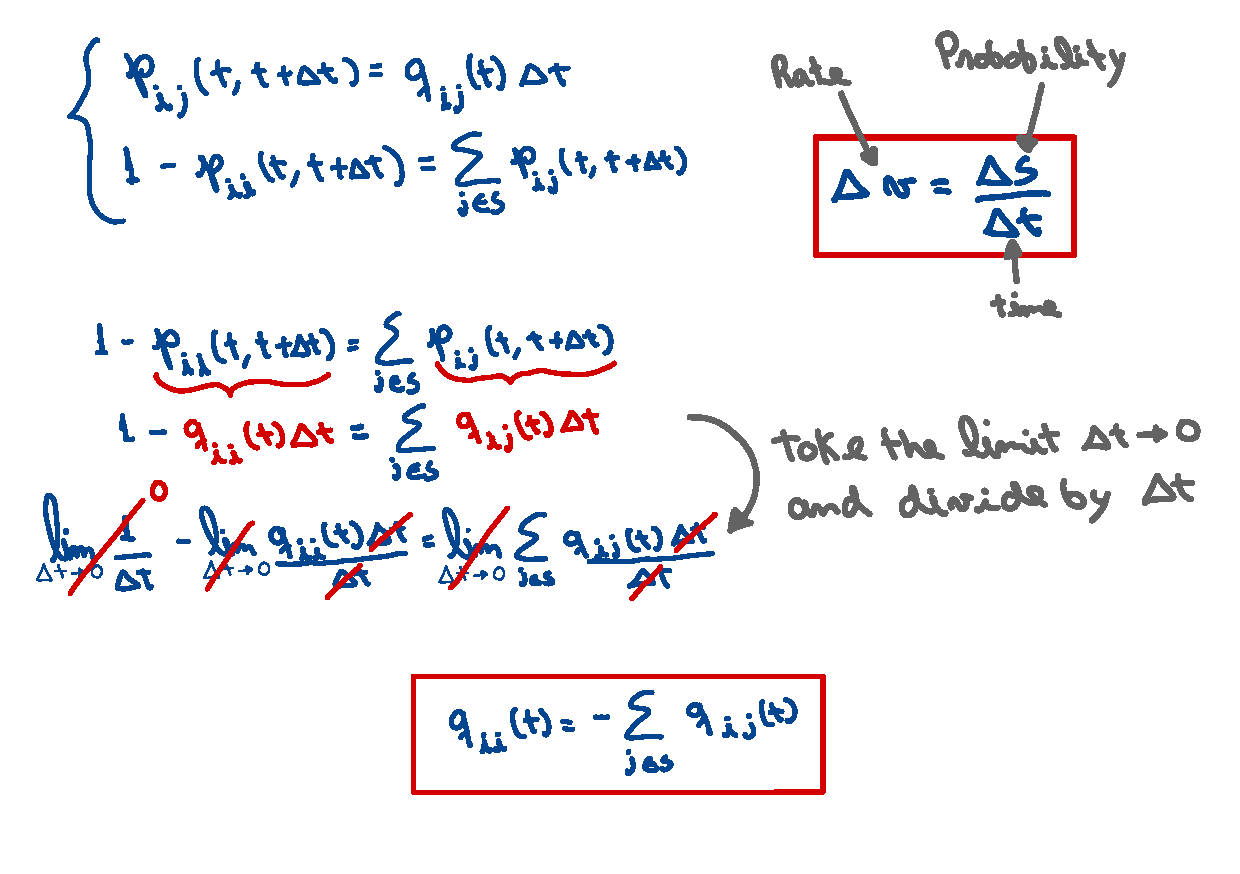
\includegraphics[width=0.95\textwidth]{slides/figures/ctmc_qt_part_one.pdf}
    \end{figure}
\end{frame}

\begin{frame}
    \frametitle{Transition Rate Matrix}
    \begin{figure}
        \centering
        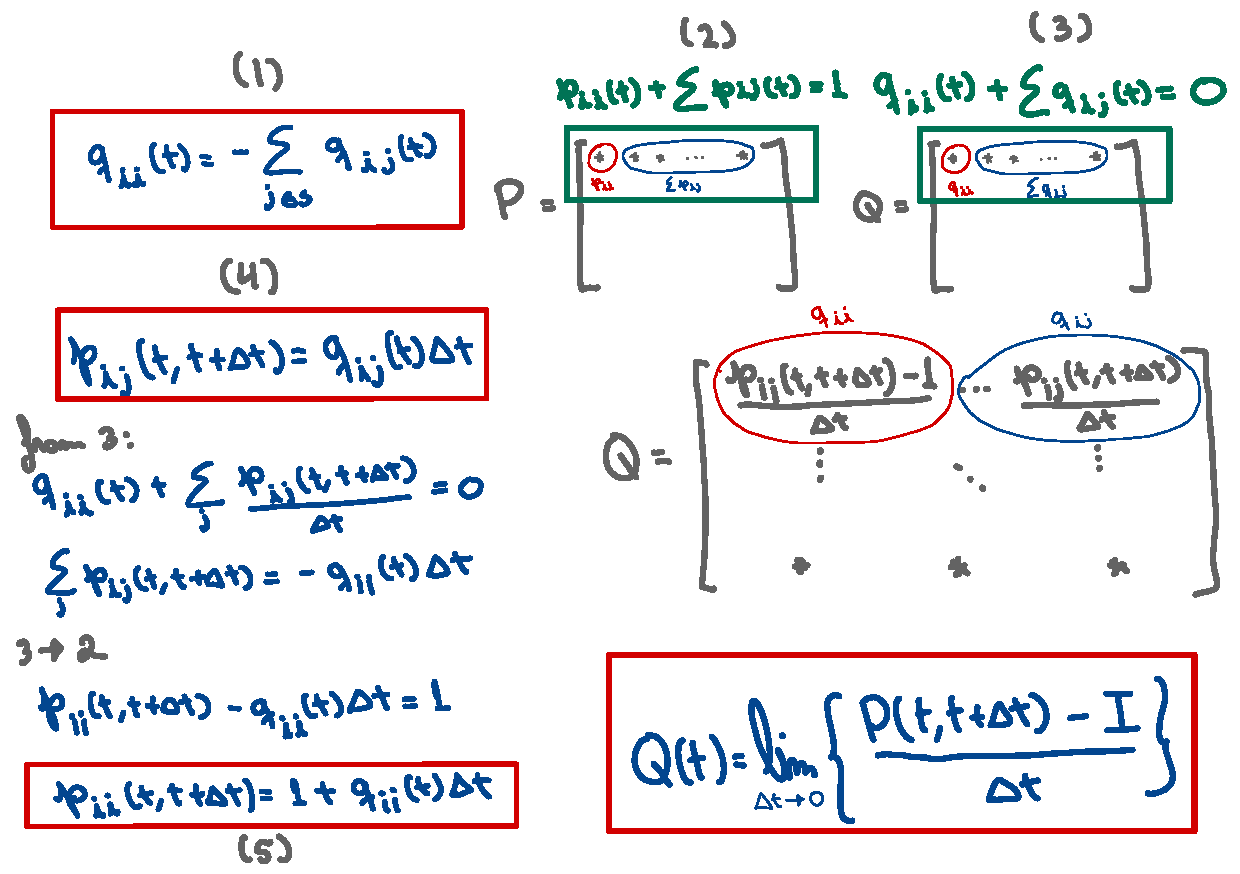
\includegraphics[width=0.95\textwidth]{slides/figures/ctmc_qt_part_two.pdf}
    \end{figure}
\end{frame}


\begin{frame}
    \frametitle{The Chapman-Kolmogorov Equations}
        \begin{itemize}
            \item The Chapman-Kolmogorov equations for a nonhomogeneous continuous-time Markov chain may be 
            obtained directly from the Markov property. They are specified by

            \small
            $$p_{ij}(s,t) = \sum_{all~k}p_{ik}(s,u)p_{kj}(u,t)~~\text{for $i$, $j = 0,1,...$ and $s\leq u\leq t$}$$

            \item When the continuous-time Markov chain is homogeneous, the Chapman-Kolmogorov equation may be written as
            \small
            $$p_{ij}(t+\Delta t) = \sum_{all~k}p_{ik}(t)p_{kj}(\Delta t)~~\text{for $t, \Delta t\geq 0$}$$

        \end{itemize}
\end{frame}

\begin{frame}
    \frametitle{The Chapman-Kolmogorov Equations (Proof)}
        \begin{figure}
            \centering
            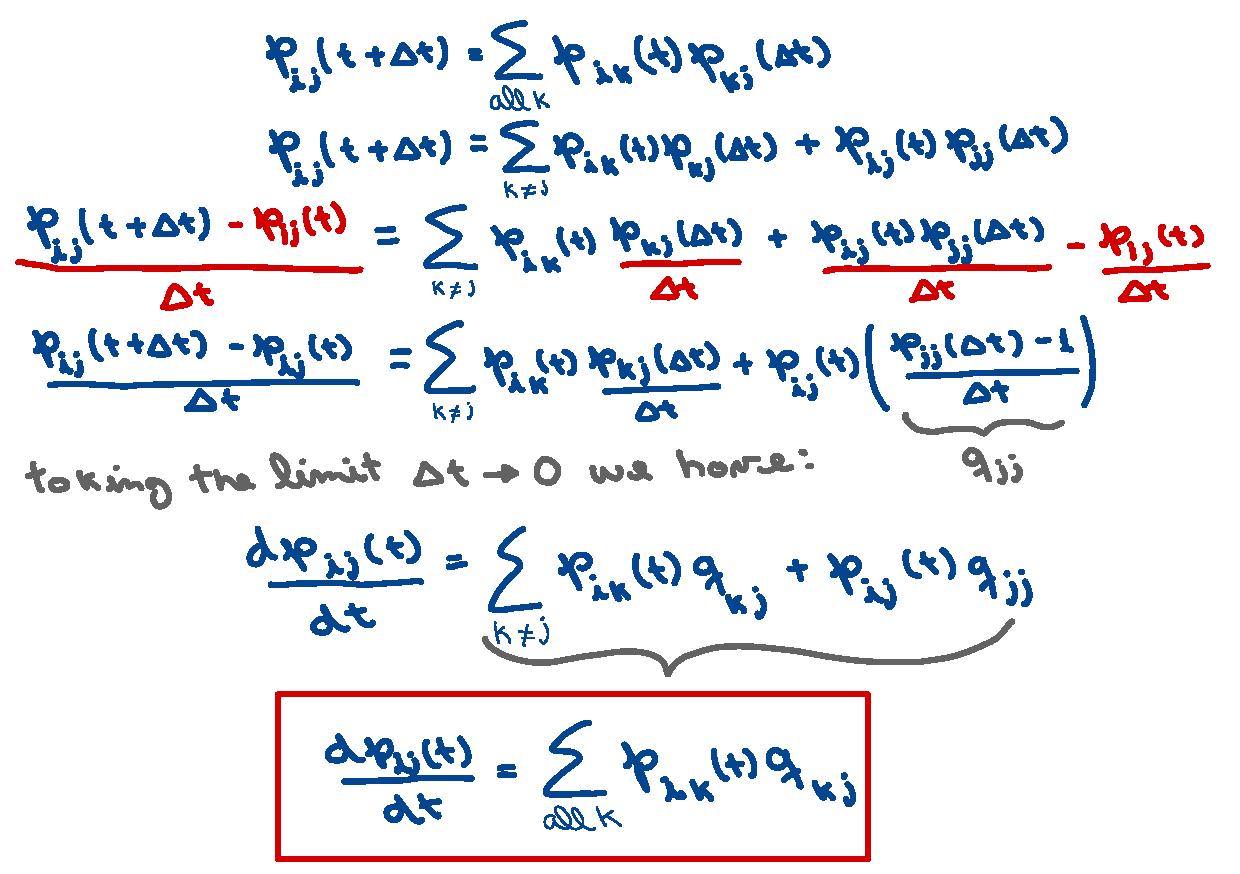
\includegraphics[width=0.95\textwidth]{slides/figures/ctmc_chapman_kolmogorov_proof.pdf}
        \end{figure}
\end{frame}

\begin{frame}
    \frametitle{The Chapman-Kolmogorov Equations}

        For a homogeneous Markov chain:

        \begin{itemize}
            \item Kolmogorov forward equation:
            $$\frac{dP_{ij}(t)}{dt} = \sum_{all~k}p_{ik}(t)q_{kj}~~{\color{red}\Rightarrow \frac{dP(t)}{dt}=P(t)Q}$$
            The solution of the forward Kolmogorov equations is given by the matrix exponencial:
            $$P(t) = ce^{Qt}~~{\color{red}\Rightarrow \frac{dP(t)}{dt} = Qce^{Qt} = QP(t)}$$
            \item Kolmogorov backward equation:
            $$\frac{dP(t)}{dt}=QP(t)$$
        \end{itemize}
\end{frame}


\begin{frame}
    \frametitle{Probability Distributions: Transient}

        \begin{itemize}

            \item \textbf{Transient distributions:} Consider a system that is modeled by a continuous-time Markov chain. 
            Let $\pi_t(t)$ be the probability that the system is in state $i$ at time $t$,

            $$\pi_i(t) = P[X(t) = i]~~{\color{red}\Rightarrow \frac{d\pi_i(t)}{dt}=\sum_{all~k}q_{ki}(t)\pi_k(t)}$$

            In matrix notation, this gives

            $$\frac{d\pi(t)}{dt} = \pi(t)Q(t)$$

            When the Markov chain is homogeneous, we may drop the dependence on time and simply write
            $$\frac{d\pi(t)}{dt} = \pi(t)Q$$

        \end{itemize}
\end{frame}

\begin{frame}
    \frametitle{Probability Distributions: Transient}

        \begin{itemize}

            \item \textbf{Transient distributions:} Consider a system that is modeled by a continuous-time Markov chain. 
            Let $\pi_t(t)$ be the probability that the system is in state $i$ at time $t$,

            $$\pi_i(t) = P[X(t) = i]~~{\color{red}\Rightarrow \frac{d\pi_i(t)}{dt}=\sum_{all~k}q_{ki}(t)\pi_k(t)}$$

            In matrix notation, this gives

            $$\frac{d\pi(t)}{dt} = \pi(t)Q(t)$$

            When the Markov chain is homogeneous, we may drop the dependence on time and simply write
            $$\frac{d\pi(t)}{dt} = \pi(t)Q$$

        \end{itemize}
\end{frame}


\begin{frame}
    \frametitle{Probability Distributions: Transient (Proof)}
    \begin{figure}
        \centering
        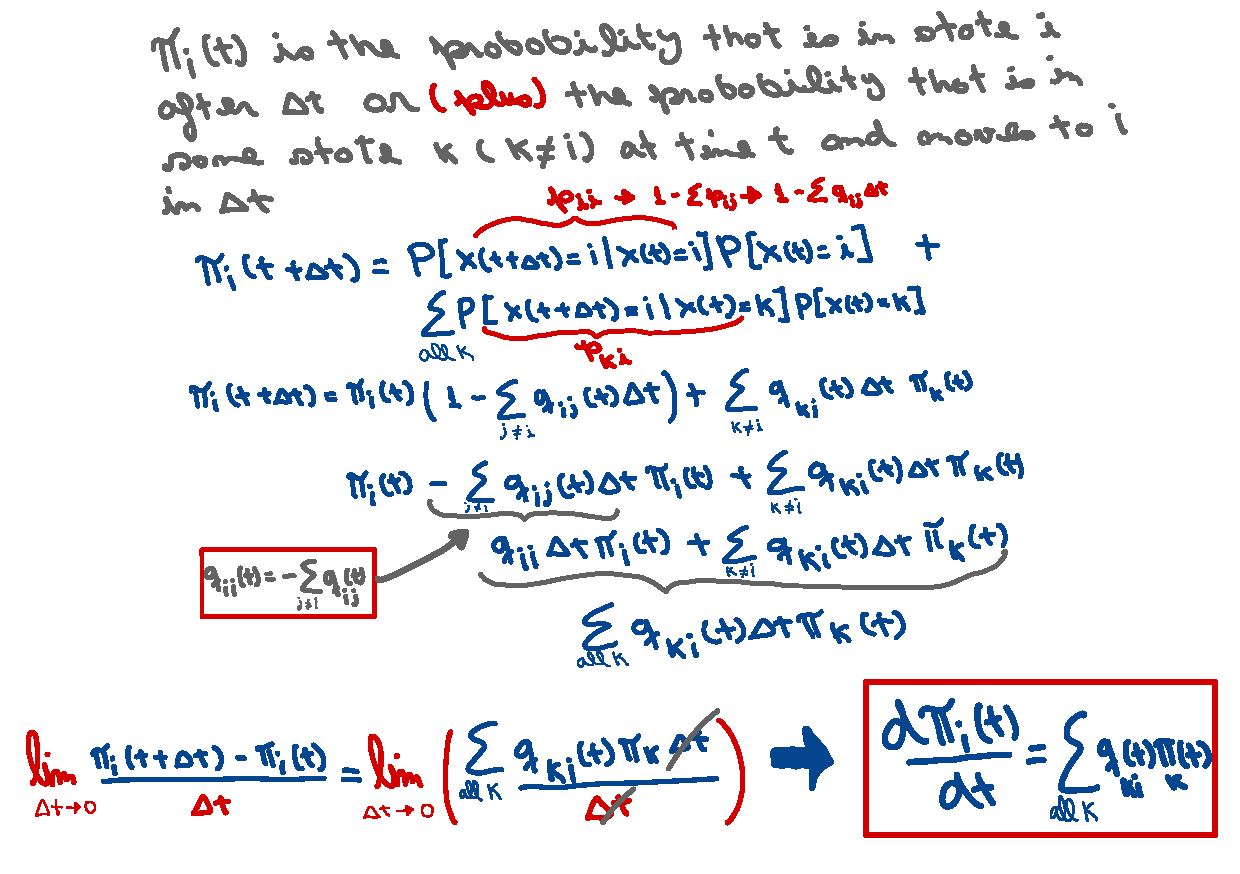
\includegraphics[width=0.95\textwidth]{slides/figures/ctmc_transient_proof.pdf}
    \end{figure}
\end{frame}


\begin{frame}
    \frametitle{Probability Distributions: Stationary}

        \begin{itemize}
            \item In a homogeneous, continuous-time Markov chain, the $i^{th}$ element of the vector $\pi_(t)$ is 
            the probability that the chain is in state $i$ at time $t$ and we have just seen that these state
            probabilities are governed by the system of differential equations
            $$\frac{d\pi(t)}{dt} = \pi(t)Q$$

            \item When the system is equilibrium (\textbf{steady-state}), there is no changes in the probability 
            distribution. In other words, the $d\pi{t}/dt$, is identically equal to zero.
            $$\pi~Q = 0$$
        \end{itemize}
\end{frame}


\begin{frame}
    \frametitle{Global Balance Equations}

        \begin{itemize}
            \item Since $|\pi| = 1$, just as in the discrete-time case, we can write the
            global balance equations. we have

            $$\sum_{all~i}\pi_i q_{ij} = 0$$
            $$\pi_j q_{jj} + \sum_{i\neq j}\pi_i q_{ij} = 0$$
            $$\sum_{i,i\neq j}\pi_i q_{ij} = \pi_j\sum_{i,i\neq j}q_{ji}$$

            \item The left-hand side represents the total flow from all states $i$, different from $j$, into 
            state $j$, while the right-hand side represents the total flow out of state $j$ into all other states $i\neq j$.

        \end{itemize}
\end{frame}


\begin{frame}
    \frametitle{Global Balance Equations: Example}
    \begin{figure}
        \centering
        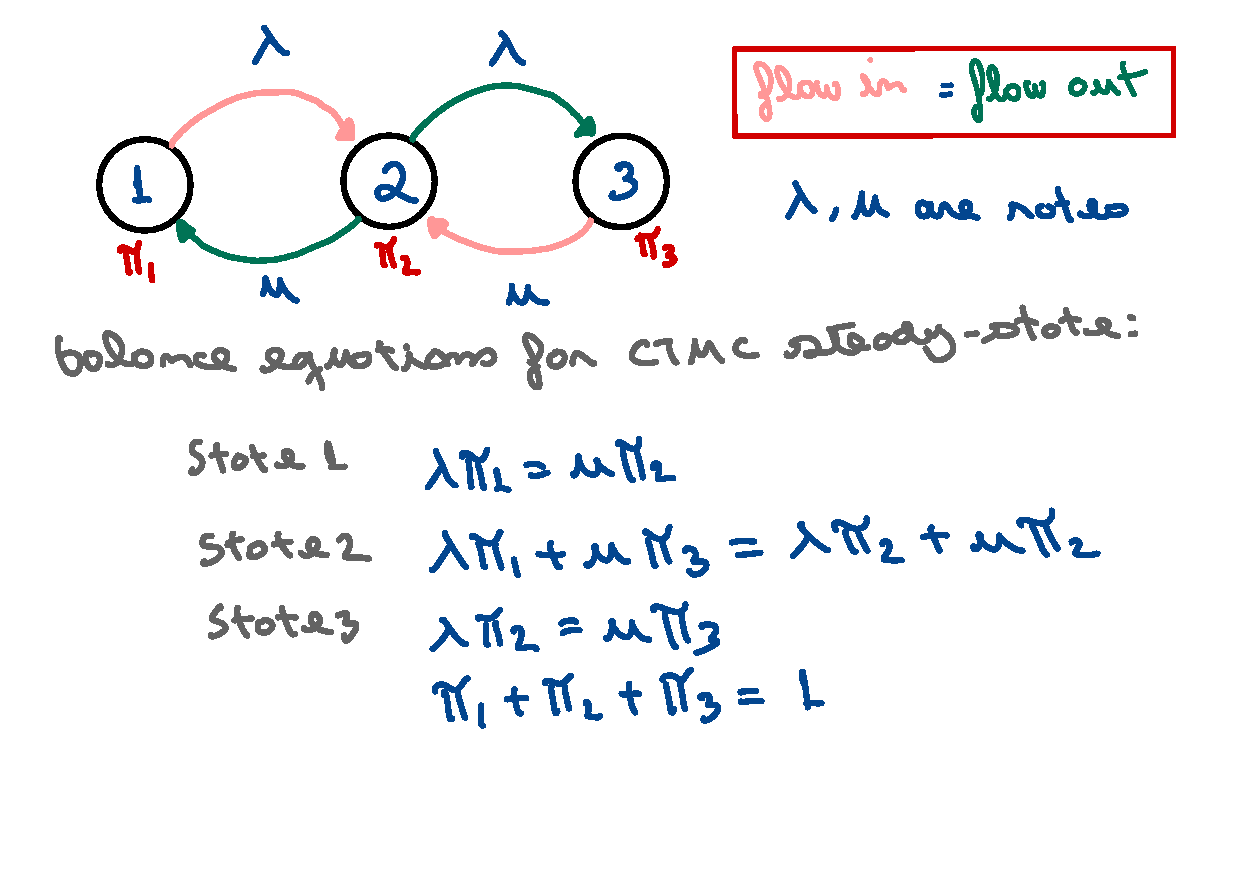
\includegraphics[width=1\textwidth]{slides/figures/ctmc_balance_equations_example.pdf}
    \end{figure}
\end{frame}

\section{Numerical Solution for Markov Chains}



\begin{frame}
    \frametitle{Numerical Solutions for Markov Chains}

        Very useful to find the stationary probabilities

        \begin{itemize}
            \item \textbf{Direct methods:}
            \begin{itemize}
                \item Gaussian elimination algorithm (linear algebra).
                %\item Grassmann, Taskar and Heyman (GTH) algorithm
            \end{itemize}
            \item \textbf{Iterative methods:}
            \begin{itemize}
                %\item Matrix powers
                \item Power method
                \item Gauss-Seidel method
            \end{itemize}
        \end{itemize}
\end{frame}



\begin{frame}
    \frametitle{Direct methods: Gaussian elimination}

        \begin{itemize}
            \item For stationary distribution of Markov chains we have:

            $$\pi Q = 0~~\text{,}\pi\geq 0~~\text{,}\sum \pi = 1$$

            \item The Gaussian elimination method will need to solve the equation:

            $$Ax = b$$

            \item To solve the Markov chain, we will need to solve

            $$Ax = Q^T\pi^T = 0 = b$$

        \end{itemize}
\end{frame}


\begin{frame}
    \frametitle{Direct methods: Gaussian elimination}

        \begin{itemize}
            \item \textbf{Step 1:} Compute for $i = 0,1,...,n-1$

            $$a_{ji} = -\frac{a_{ji}}{a_{ii}}~~\text{, $j>i$}$$
            $$a_{jk} = a_{jk}+a_{ji}a_{ik}~~\text{, $j,k>i$}$$

            \item \textbf{Step 2:} Set $x_{n} = 1$ and compute for $i = n-1, n-2,...,0$

            $$x_i = -\left[\sum_{j=i+1}^n a_{ij}x_{j}\right]/a_{ii}$$

            \item \textbf{Step 3:} Compute for $i = 0,1,...,n$

            $$\pi_i = \frac{x_i}{\sum_{j=0}^n x_j}$$

        \end{itemize}
\end{frame}

\begin{frame}
    \frametitle{Direct methods: Gaussian elimination}
    \begin{figure}
        \centering
        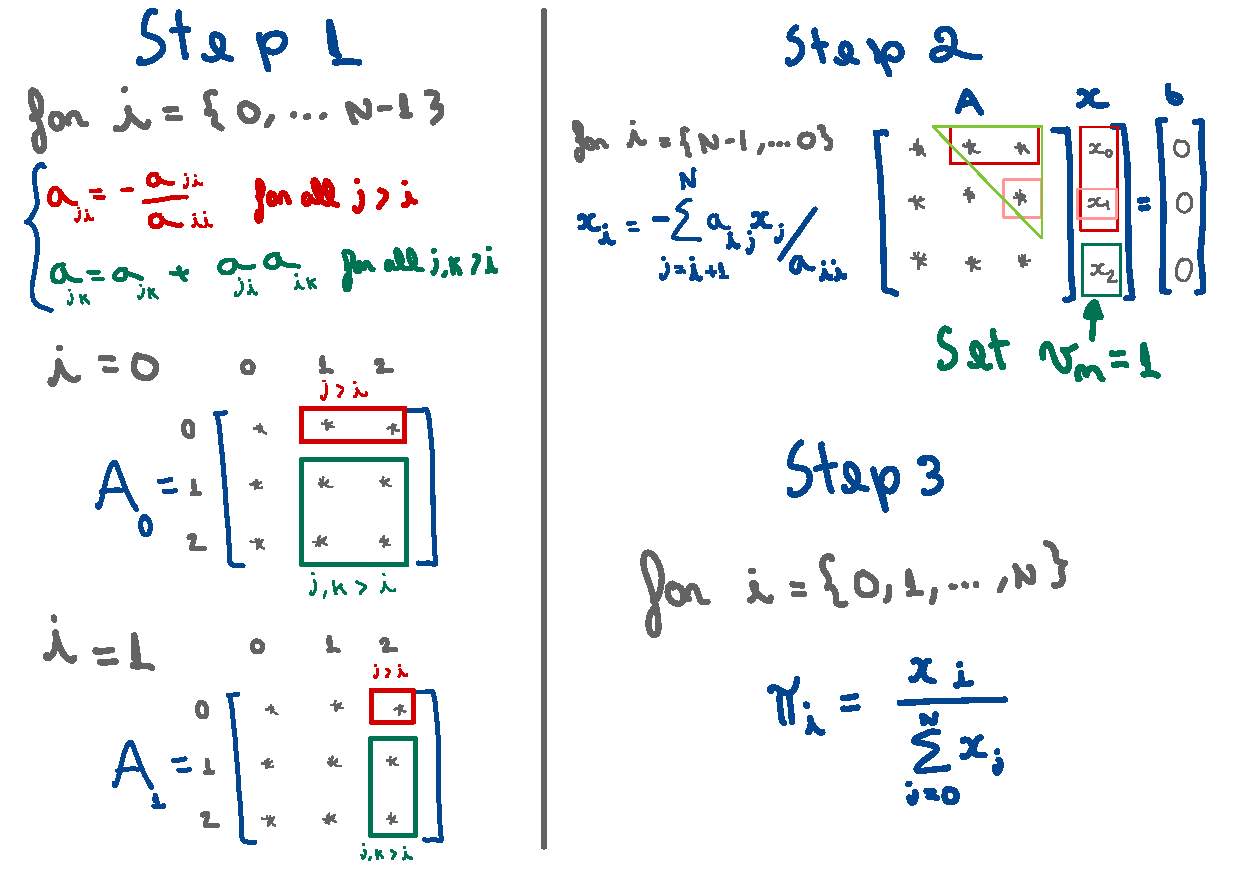
\includegraphics[width=0.95\textwidth]{slides/figures/gaussian_elimination_method.pdf}
    \end{figure}
\end{frame}

\begin{frame}
    \frametitle{Direct methods: Gaussian elimination}

        \begin{itemize}
            \item The operation required to solve the equilibrium equation involve subtractions
            which may cause a loss of high order precision

            \item For Gaussian elimination the complexity is $O(N^3)$

            \item Only practical when $N$ is not too large (e.g., $N\leq1000$)

            \item In practice, \textbf{large matrices are often space} (i.e., many zeros). This
            property is exploited by iterative methods

        \end{itemize}
\end{frame}



\begin{frame}
    \frametitle{Iterative methods: The Power Method}

 

        \begin{itemize}

            \item Perhaps the approach that first comes to mind when we need to find the stationary 
            distribution of an finite, ergodic, DTMC, is to let the chain evolve 
            over time, step by step, until it reaches its \textbf{stationary distribution} where            
            
            $$\pi = \pi P$$

            \item Choose an initial\footnote{
                When the Markov chain is finite, aperiodic, and irreducible, the vectors $\pi^k$
                converge to the stationary probability vector π regardless of the choice of initial vector.} probability 
                distribution $\pi^0$,and compute for $n=0,1,...$

            $$\pi^{k+1} = \pi^{k} P$$

            until $|\pi^{k+1} - \pi^k|$ is small

        \end{itemize}
\end{frame}


\begin{frame}
    \frametitle{Iterative methods: Gauss-Seidel method}

 

        \begin{itemize}

            \item It is a variant of the \textbf{power method}. 

            \item \textbf{Power method}: Computes recursivelly the values of $\pi^{k+1}$ from $\pi^{k+1} = \pi^k P$

            $$\pi_{i}^{k+1} = \sum_{j=0}^{N} p_{j}^k p_{ji}$$


            \item \textbf{Gauss-Seidel method}: The convergence is \textbf{much faster} than power method.

            $$\pi_{i}^{k+1} = \sum_{j=0}^{i} \pi_{j}^{k+1} p_{ji} + \sum_{j=i+1}^N \pi_{j}^{k}p_{ji}$$ 


        \end{itemize}
\end{frame}

